%%
%% This is file `sample__1col.tex',
%% generated with the docstrip utility.
%%
%% The original source files were:
%%
%% sample.dtx  (with options: `all,1col,listings')
%% 
%%
%% The first command in your LaTeX source must be the \documentclass command.
%%
%% Options:
%% twocolumn : Two column layout.
%% hf: enable header and footer.
\documentclass[%
]{ceurart}

%%
%% One can fix some overfulls
\sloppy

%% Listings support
\usepackage{listings}
%% auto break lines
\lstset{breaklines=true}

%% end of the preamble, start of the body of the document source.
\begin{document}

%%
%% Rights management information.
%% CC-BY is default license.
\copyrightyear{2024}
\copyrightclause{Copyright for this paper by its authors.
  Use permitted under Creative Commons License Attribution 4.0
  International (CC BY 4.0).}

%%
%% This command is for the conference information
\conference{Woodstock'24: Symposium on the irreproducible science,
  June 10--14, 2024, Woodstock, NY}

%%
%% The "title" command
\title{A better way to format your document for CEUR-WS}

\tnotemark[1]
\tnotetext[1]{You can use this document as the template for preparing your publication. We recommend using the latest version of the ceurart style.}

%%
%% The "author" command and its associated commands are used to define
%% the authors and their affiliations.
\author[1,2]{Dmitry S. Kulyabov}[%
orcid=0000-0002-0877-7063,
email=kulyabov-ds@rudn.ru,
url=https://yamadharma.github.io/,
]
\cormark[1]
\fnmark[1]
\address[1]{RUDN University,
  6 Miklukho-Maklaya St, Moscow, 117198, Russian Federation}
\address[2]{Joint Institute for Nuclear Research,
  6 Joliot-Curie St, Dubna, 141980, Russian Federation}

\author[3]{Ilaria Tiddi}[%
orcid=0000-0001-7116-9338,
email=i.tiddi@vu.nl,
url=https://kmitd.github.io/ilaria/,
]
\fnmark[1]
\address[3]{Vrije Universiteit Amsterdam, De Boelelaan 1105, 1081 HV Amsterdam, The Netherlands}

\author[4]{Manfred Jeusfeld}[%
orcid=0000-0002-9421-8566,
email=Manfred.Jeusfeld@acm.org,
url=http://conceptbase.sourceforge.net/mjf/,
]
\fnmark[1]
\address[4]{University of Skövde, Högskolevägen 1, 541 28 Skövde, Sweden}

%% Footnotes
\cortext[1]{Corresponding author.}
\fntext[1]{These authors contributed equally.}

%%
%% The abstract is a short summary of the work to be presented in the
%% article.
\begin{abstract}
  A clear and well-documented \LaTeX{} document is presented as an article formatted for publication by CEUR-WS in a conference proceedings.
  Based on the \enquote{ceurart} document class, this article presents and explains many of the common variations, as well as many of the formatting elements an author may use in the preparation of the documentation of their work.
\end{abstract}

%%
%% Keywords. The author(s) should pick words that accurately describe
%% the work being presented. Separate the keywords with commas.
\begin{keywords}
  LaTeX class \sep
  paper template \sep
  paper formatting \sep
  CEUR-WS
\end{keywords}

%%
%% This command processes the author and affiliation and title
%% information and builds the first part of the formatted document.
\maketitle

\section{Introduction}

CEUR-WS's article template provides a consistent \LaTeX{} style for use across CEUR-WS publications, and incorporates accessibility and metadata-extraction functionality.
This document will explain the major features of the document class.

If you are new to publishing with CEUR-WS, this document is a valuable guide to the process of preparing your work for publication.

The ``\verb|ceurart|'' document class can be used to prepare articles for any CEUR-WS publication, and for any stage of publication, from review to final ``camera-ready'' copy with {\itshape very} few changes to the source.

This class depends on the following packages for its proper functioning:

\begin{itemize}
\item
\verb|natbib.sty|
 for citation processing;
\item
\verb|geometry.sty|
 for margin settings;
\item
\verb|graphicx.sty|
 for graphics inclusion;
\item
\verb|hyperref.sty|
 optional package if hyperlinking is required in the document;
\item
\verb|fontawesome5.sty|
 optional package for bells and whistles.
\end{itemize}

All the above packages are part of any standard \LaTeX{} installation. Therefore, the users need not be bothered about downloading any extra packages.

\section{Modifications}

Modifying the template---including but not limited to: adjusting margins, typeface sizes, line spacing, paragraph and list definitions, and the use of the
\verb|\vspace|
 command to manually adjust the vertical spacing between elements of your work---is not allowed.

\section{Template parameters}

There are a number of template parameters which modify some part of the
\verb|ceurart|
 document class.
This parameters are enclosed in square brackets and are a part of the
\verb|\documentclass|
 command:
\begin{lstlisting}[language={[latex]TeX}]
\documentclass[parameter]{ceurart}
\end{lstlisting}

Frequently-used parameters, or combinations of parameters, include:
\begin{itemize}
\item
\verb|twocolumn|
 : Two column layout.
\item
\verb|hf|
 : Enable header and footer\footnote{You can enable the display of page numbers in the final version of the entire collection. In this case, you should adhere to the end-to-end pagination of individual papers.}.
\end{itemize}

\section{Front matter}

\subsection{Title Information}

The titles of papers should be either all use the emphasizing capitalized style or they should all use the regular English (or native language) style.
It does not make a good impression if you or your authors mix the styles.

Use the
\verb|\title|
command to define the title of your work. Do not insert line breaks in your title.

\subsection{Title variants}

\verb|\title|
command have the below options:
\begin{itemize}
\item
\verb|title|
: Document title. This is default option.
\begin{lstlisting}[language={[latex]TeX}]
\title[mode=title]{This is a title}
\end{lstlisting}

You can just omit it, like as follows:
\begin{lstlisting}[language={[latex]TeX}]
\title{This is a title}
\end{lstlisting}

\item
\verb|alt|
: Alternate title.
\begin{lstlisting}[language={[latex]TeX}]
\title[mode=alt]{This is a alternate title}
\end{lstlisting}

\item
\verb|sub|
: Sub title.
\begin{lstlisting}[language={[latex]TeX}]
\title[mode=sub]{This is a sub title}
\end{lstlisting}
You can just use
\verb|\subtitle|
 command, as follows:
\begin{lstlisting}[language={[latex]TeX}]
\subtitle{This is a sub title}
\end{lstlisting}

\item
\verb|trans|
: Translated title.
\begin{lstlisting}[language={[latex]TeX}]
\title[mode=trans]{This is a translated title}
\end{lstlisting}

\item
\verb|transsub|
: Translated sub title.
\begin{lstlisting}[language={[latex]TeX}]
\title[mode=transsub]{This is a translated sub title}
\end{lstlisting}
\end{itemize}

\subsection{Authors and Affiliations}

Each author must be defined separately for accurate metadata identification.
Multiple authors may share one affiliation.
Authors' names should not be abbreviated; use full first names wherever possible.
Include authors' e-mail addresses whenever possible.

\verb|\author|
command have the below options:
\begin{itemize}
\item
\verb|style|
 : Style of author name (chinese)
\item
\verb|prefix|
 : Prefix
\item
\verb|suffix|
 : Suffix
\item
\verb|degree|
 : Degree
\item
\verb|role|
 : Role
\item
\verb|orcid|
 : ORCID
\item
\verb|email|
 : E-mail
\item
\verb|url|
 : URL
\end{itemize}

Author names can have some kinds of marks and notes:
\begin{itemize}
\item affiliation mark:
\verb|\author[<num>]|
.
\end{itemize}

The author names and affiliations could be formatted in two ways:
\begin{enumerate}
\item Group the authors per affiliation.
\item Use an explicit mark to indicate the affiliations.
\end{enumerate}

Author block example:
\begin{lstlisting}[language={[latex]TeX}]
\author[1,2]{Author Name}[%
    prefix=Prof.,
    degree=D.Sc.,
    role=Researcher,
    orcid=0000-0000-000-0000,
    email=name@example.com,
    url=https://name.example.com
]

\address[1]{Affiliation #1}
\address[2]{Affiliation #2}
\end{lstlisting}

\subsection{Abstract and Keywords}

Abstract shall be entered in an environment that starts with
\verb|\begin{abstract}|
 and ends with
\verb|\end{abstract}|
.

\begin{lstlisting}[language={[latex]TeX}]
\begin{abstract}
  This is an abstract.
\end{abstract}
\end{lstlisting}

The key words are enclosed in a
\verb|keywords|
environment. Use
\verb|\sep|
 to separate keywords.

\begin{lstlisting}[language={[latex]TeX}]
\begin{keywords}
  First keyword \sep
  Second keyword \sep
  Third keyword \sep
  Fourth keyword
\end{keywords}
\end{lstlisting}

At the end of front matter add
\verb|\maketitle|
 command.

\subsection{Various Marks in the Front Matter}

The front matter becomes complicated due to various kinds of notes and marks to the title and author names.
Marks in the title will be denoted by a star ($\star$) mark; footnotes are denoted by super scripted Arabic numerals, corresponding author by an Conformal asterisk (
\verb|*|
) mark.

\subsubsection{Title marks}

Title mark can be entered by the command,
\verb|\tnotemark[<num>]|
and the corresponding text can be entered with the command
\verb|\tnotetext[<num>]{<text>}|.

An example will be:
\begin{lstlisting}[language={[latex]TeX}]
\title{A better way to format your document for CEUR-WS}

\tnotemark[1]
\tnotetext[1]{You can use this document as the template for preparing your publication. We recommend using the latest version of the ceurart style.}
\end{lstlisting}

\verb|\tnotemark|
 and
\verb|\tnotetext|
 can be anywhere in the front matter, but should be before
\verb|\maketitle|
 command.

\subsubsection{Author marks}

Author names can have some kinds of marks and notes:
\begin{itemize}
\item footnote mark :
\verb|\fnmark[<num>]|

\item footnote text :
\verb|\fntext[<num>]{<text>}|

\item corresponding author mark :
\verb|\cormark[<num>]|

\item corresponding author text :
\verb|\cortext[<num>]{<text>}|

\end{itemize}

\subsubsection{Other marks}

At times, authors want footnotes which leave no marks in the author names. The note text shall be listed as part of the front matter notes. Class files provides
\verb|\nonumnote|
 for this purpose. The usage
\begin{lstlisting}[language={[latex]TeX}]
\nonumnote{<text>}
\end{lstlisting}
and should be entered anywhere before the
\verb|\maketitle|
 command for this to take effect.

\section{Sectioning Commands}

Your work should use standard \LaTeX{} sectioning commands:
\verb|\section|%
,
\verb|\subsection|%
,
\verb|\subsubsection|%
, and
\verb|\paragraph|%
.
They should be numbered; do not remove the numbering from the commands.

Simulating a sectioning command by setting the first word or words of a paragraph in boldface or italicized text is not allowed.

\section{Tables}

The
\verb|ceurart|
document class includes the
\verb|booktabs|
package---\url{https://ctan.org/pkg/booktabs}---for preparing high-quality tables.

Table captions are placed \textit{above} the table.

Because tables cannot be split across pages, the best placement for them is typically the top of the page nearest their initial cite. To ensure this proper ``floating'' placement of tables, use the environment
\verb|table|
to enclose the table's contents and the table caption. The contents of the table itself must go in the
\verb|tabular|
environment, to be aligned properly in rows and columns, with the desired horizontal and vertical rules.

Immediately following this sentence is the point at which Table~\ref{tab:freq} is included in the input file; compare the placement of the table here with the table in the printed output of this document.

\begin{table*}
  \caption{Frequency of Special Characters}
  \label{tab:freq}
  \begin{tabular}{ccl}
    \toprule
    Non-English or Math&Frequency&Comments\\
    \midrule
    \O & 1 in 1,000& For Swedish names\\
    $\pi$ & 1 in 5& Common in math\\
    \$ & 4 in 5 & Used in business\\
    $\Psi^2_1$ & 1 in 40,000& Unexplained usage\\
    \bottomrule
  \end{tabular}
\end{table*}

To set a wider table, which takes up the whole width of the page's live area, use the environment
\verb|table*|
to enclose the table's contents and the table caption.  As with a single-column table, this wide table will
\enquote{float}
to a location deemed more desirable.
Immediately following this sentence is the point at which Table~\ref{tab:commands} is included in the input file; again, it is instructive to compare the placement of the table here with the table in the printed output of this document.

\begin{table}
  \caption{Some Typical Commands}
  \label{tab:commands}
  \begin{tabular}{ccl}
    \toprule
    Command &A Number & Comments\\
    \midrule
    \texttt{{\char'134}author} & 100& Author \\
    \texttt{{\char'134}table}& 300 & For tables\\
    \texttt{{\char'134}table*}& 400& For wider tables\\
    \bottomrule
  \end{tabular}
\end{table}

\section{Math Equations}

You may want to display math equations in three distinct styles: inline, numbered or non-numbered display.
Each of the three are discussed in the next sections.

\subsection{Inline (In-text) Equations}

A formula that appears in the running text is called an inline or in-text formula.
It is produced by the
\verb|math|
environment, which can be invoked with the usual
\verb|\begin|
\ldots{}
\verb|\end|
construction or with the short form
\verb|$|
\ldots{}
\verb|$|%
.
You can use any of the symbols and structures, from $\alpha$ to $\omega$, available in \LaTeX~\cite{Lamport:LaTeX}; this section will simply show a few examples of in-text equations in context.
Notice how this equation:
\begin{math}
  \lim_{n\rightarrow \infty} \frac{1}{n} = 0,
\end{math}
set here in in-line math style, looks slightly different when set in display style.
(See next section).

\subsection{Display Equations}

A numbered display equation---one set off by vertical space from the text and centered horizontally---is produced by the
\verb|equation|
environment.
An unnumbered display equation is produced by the
\verb|displaymath|
environment.

Again, in either environment, you can use any of the symbols and structures available in \LaTeX{}; this section will just give a couple of examples of display equations in context.
First, consider the equation, shown as an inline equation above:
\begin{equation}
  \lim_{n\rightarrow \infty} \frac{1}{n} = 0.
\end{equation}
Notice how it is formatted somewhat differently in the
\verb|displaymath|
environment.
Now, we'll enter an unnumbered equation:
\begin{displaymath}
  S_{n} = \sum_{i=1}^{n} x_{i} ,
\end{displaymath}
and follow it with another numbered equation:
\begin{equation}
  \lim_{x \to 0} (1 + x)^{1/x} = e
\end{equation}
just to demonstrate \LaTeX's able handling of numbering.

\section{Figures}

The
\verb|figure|
environment should be used for figures.
One or more images can be placed within a figure.
If your figure contains third-party material, you must clearly identify it as such, as shown in the example below.

\begin{figure}
  \centering
  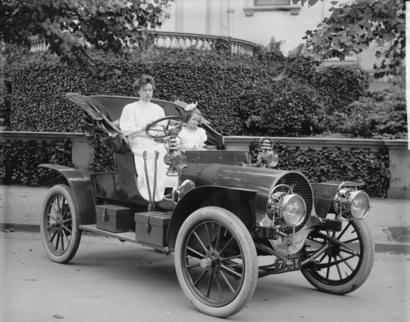
\includegraphics[width=\linewidth]{sample-franklin}
  \caption{1907 Franklin Model D roadster. Photograph by Harris \&
    Ewing, Inc. [Public domain], via Wikimedia
    Commons. (\url{https://goo.gl/VLCRBB}).}
\end{figure}

Your figures should contain a caption which describes the figure to the reader.
Figure captions go below the figure. Your figures should also include a description suitable for screen readers, to assist the visually-challenged to better understand your work.

Figure captions are placed below the figure.

\section{Citations and Bibliographies}

The use of Bib\LaTeX{} for the preparation and formatting of one's references is strongly recommended.
Authors' names should be complete---use full first names (``Donald E. Knuth'') not initials (``D. E. Knuth'')---and the salient identifying features of a reference should be included: title, year, volume, number, pages, article DOI, etc.

The bibliography is included in your source document with these two commands, placed just before the
\verb|\end{document}|
command:
\begin{lstlisting}[language={[latex]TeX}]
\bibliography{bibfile}
\end{lstlisting}
where
\verb|bibfile|
 is the name, without the
\verb|.bib|
suffix, of the Bib\TeX{} file.

\subsection{Some examples}

A paginated journal article \cite{Abril07}, an enumerated journal
article \cite{Cohen07}, a reference to an entire issue
\cite{JCohen96}, a monograph (whole book) \cite{Kosiur01}, a
monograph/whole book in a series (see 2a in spec. document)
\cite{Harel79}, a divisible-book such as an anthology or compilation
\cite{Editor00} followed by the same example, however we only output
the series if the volume number is given \cite{Editor00a} (so series
should not be present since it has no vol. no.), a chapter in a
divisible book \cite{Spector90}, a chapter in a divisible book in a
series \cite{Douglass98}, a multi-volume work as book \cite{Knuth97},
an article in a proceedings (of a conference, symposium, workshop for
example) (paginated proceedings article) \cite{Andler79}, a
proceedings article with all possible elements \cite{Smith10}, an
example of an enumerated proceedings article \cite{VanGundy07}, an
informally published work \cite{Harel78}, a doctoral dissertation
\cite{Clarkson85}, a master's thesis: \cite{anisi03}, an online
document / world wide web resource \cite{Thornburg01, Ablamowicz07,
  Poker06}, a video game (Case 1) \cite{Obama08} and (Case 2)
\cite{Novak03} and \cite{Lee05} and (Case 3) a patent
\cite{JoeScientist001}, work accepted for publication \cite{rous08},
prolific author \cite{SaeediMEJ10} and \cite{SaeediJETC10}. Other
cites might contain `duplicate' DOI and URLs (some SIAM articles)
\cite{Kirschmer:2010:AEI:1958016.1958018}. Multi-volume works as books
\cite{MR781536} and \cite{MR781537}. A couple of citations with DOIs:
\cite{2004:ITE:1009386.1010128,Kirschmer:2010:AEI:1958016.1958018}. Online
citations: \cite{TUGInstmem, Thornburg01, R, UMassCitations}.

\section{Ethical disclaimers}

A disclaimer is a note of disclaimer of responsibility~\cite{kulyabov_2024_editorial_author-ethics_en}.
For example, authors' statements about conflicts of interest, author contributions, acknowledgements, etc.

Authors should not prepare these disclaimers as a numbered or unnumbered
\verb|\section|%
; please use the special environments instead.

\subsection{Author contributions}

The Committee on Publication Ethics (COPE) draws attention to the problem of authorship \cite{cope_book_authorship_en}.
The CRediT system (\url{https://credit.niso.org/}) is proposed to formalize author roles.
The CRediT (Contributor Roles Taxonomy) offers 14 possible author roles \cite{holcombe_2019_contributorship-not-authorship_en}.
This is not really a taxonomy, but a faceted classification. Author roles are not always independent in themselves.

The following statements should be used \emph{Conceptualization, X.X. and Y.Y.; methodology, X.X.; software, X.X.; validation, X.X., Y.Y. and Z.Z.; formal analysis, X.X.; investigation, X.X.; resources, X.X.; data curation, X.X.; writing---original draft preparation, X.X.; writing---review and editing, X.X.; visualization, X.X.; supervision, X.X.; project administration, X.X.; funding acquisition, Y.Y.}
Please add at the end of the statement:
\emph{All authors have read and agreed to the published version of the manuscript.}

This section has a special environment:
\begin{lstlisting}[language={[latex]TeX}]
\begin{authorcontributions}
…
\end{authorcontributions}
\end{lstlisting}

\subsection{Funding}

Disclaimer \emph{funding} refers primarily to external funding if the research was externally initiated.
If the research is entirely the initiative of the author's team, it is better to indicate gratitude for partial funding of some of the stages of the research in the \emph{Acknowledgments} section.
The fact that the author's team has received external funding should be recorded in the disclaimer as a matter of course.
When mentioning the sponsor, its exact data (name of the organization, grant number, etc.) and the country of its location should be specified (for example \emph{This research was funded by NAME OF FUNDER grant number XXX}).
If there is any support, it is recommended to clarify in the \emph{Conflicts of interest} section at which stages of the research and how the support was used.
If there is no external funding, it is written: \emph{This research received no external funding}.
If it is impossible to obtain information from the authors about the source of funding, then write: \emph{Not specified}.

This section has a special environment:
\begin{lstlisting}[language={[latex]TeX}]
\begin{funding}
…
\end{funding}
\end{lstlisting}

\subsection{Data availability statement}

Data are particularly important in reproducible researches.
The data availability statement tells the reader where the research data related to the article are located and under what conditions the data can be accessed.
References to the dataset are also provided.

If no new data is created or analyzed, please write:
\emph{No new data were created or analyzed in this study. Data sharing is not applicable.}

This section has a special environment:
\begin{lstlisting}[language={[latex]TeX}]
\begin{dataavailability}
…
\end{dataavailability}
\end{lstlisting}

\subsection{Conflicts of interest}

This disclaimer must be included.

Conflicts of interest can comment on various aspects, but usually the author's past or current employment is indicated.
Grants (especially from for-profit companies) received not only by the author but also by the organization for which he or she works are indicated.
If the author is associated with a sponsor, it is indicated where the research was conducted.

If there is no conflict of interest, then the corresponding statement should also be included: \emph{The authors declare no conflict of interest}.

This section has a special environment:
\begin{lstlisting}[language={[latex]TeX}]
\begin{conflictsofinterest}
…
\end{conflictsofinterest}
\end{lstlisting}

\subsection{Acknowledgments}

Identification of funding sources and other support, and thanks to individuals and groups that assisted in the research and the preparation of the work should be included in an acknowledgment section, which is placed just before the reference section in your document.

This section has a special environment:
\begin{lstlisting}[language={[latex]TeX}]
\begin{acknowledgments}
These are different acknowledgments.
\end{acknowledgments}
\end{lstlisting}
so that the information contained therein can be more easily collected during the article metadata extraction phase, and to ensure consistency in the spelling of the section heading.

\subsection{Declaration on Generative AI}

  Either:
\emph{The author(s) have not employed any Generative AI tools.}\\
  or (by using the activity taxonomy in \url{https://ceur-ws.org/genai-tax.html}):
\emph{During the preparation of this work, the author(s) used X-GPT-4 and Gramby in order to: Grammar
and spelling check. Further, the author(s) used X-AI-IMG for figures 3 and 4 in order to: Generate
images. After using these tool(s)/service(s), the author(s) reviewed and edited the content as
needed and take(s) full responsibility for the publication’s content.}

This section has a special environment:
\begin{lstlisting}[language={[latex]TeX}]
\begin{aideclaration}
…
\end{aideclaration}
\end{lstlisting}

\section{Appendices}

If your work needs an appendix, add it before the
\verb|\end{document}|
command at the conclusion of your source document.

Start the appendix with the
\verb|\appendix|
command:
\begin{lstlisting}[language={[latex]TeX}]
\appendix
\end{lstlisting}
and note that in the appendix, sections are lettered, not numbered.

\vspace{\baselineskip}

\begin{authorcontributions}
  Conceptualization, Manfred Jeusfeld and Ilaria Tiddi; methodology, Manfred Jeusfeld; writing---original draft preparation, Dmitry S. Kulyabov; writing---review and editing, Manfred Jeusfeld.
  All authors have read and agreed to the published version of the manuscript.
\end{authorcontributions}

\begin{funding}
    This research received no external funding.
\end{funding}

\begin{dataavailability}
    No new data were created or analysed during this study. Data sharing is not applicable.
\end{dataavailability}

\begin{conflictsofinterest}
    The authors declare no conflict of interest.
\end{conflictsofinterest}

%%
%% The acknowledgments section is defined using the "acknowledgments" environment
%% (and NOT an unnumbered section). This ensures the proper
%% identification of the section in the article metadata, and the
%% consistent spelling of the heading.
\begin{acknowledgments}
Thanks to the developers of ACM consolidated LaTeX styles \url{https://github.com/borisveytsman/acmart} and to the developers of Elsevier updated \LaTeX{} templates \url{https://www.ctan.org/tex-archive/macros/latex/contrib/els-cas-templates}.
\end{acknowledgments}

\begin{aideclaration}
    The authors have not employed any Generative AI tools.
\end{aideclaration}

%%
%% Define the bibliography file to be used
\bibliography{sample-ceur}

%%
%% If your work has an appendix, this is the place to put it.
\appendix

\section{Online Resources}

The sources for the ceur-art style are available via
\begin{itemize}
\item \href{https://github.com/yamadharma/ceurart}{GitHub},
\item \href{https://www.overleaf.com/latex/templates/template-for-submissions-to-ceur-workshop-proceedings-ceur-ws-dot-org/pkfscdkgkhcq}{Overleaf template}.
\end{itemize}

\section{\TeX{}Live distribution}

While latex is a fairly stable application, the same cannot always be attributed to specific \LaTeX{} distributions.
We suggest using the \TeX{}Live distribution.
\TeX{}Live is the most complete distribution of \LaTeX{} supported by the \TeX{} community.
It supports a large number of operating systems.
It has been in development since 1996.
It was based on the te\TeX{} distribution.
MacTeX is a variant of the \TeX{}Live distribution for macOS.
\TeX{}Live is a distribution with continuous updates as part of an annual version of the distribution.
The main page of the \TeX{}Live distribution is \url{https://www.tug.org/texlive/}.
The \TeX{}Live distribution is the basis for the Overleaf online service.

The \TeX{}Live distribution contains all the necessary packages, programs, fonts.

It is recommended to use the lualatex format to compile documents for CEUR-WS.

\subsection{Installing \TeX{}Live with the package manager}

For Linux-based systems, use the standard installation methods via the distribution's package manager.
For Windows, use the Chocolatey package manager (\url{https://chocolatey.org/}):
\begin{lstlisting}[language=sh]
choco install texlive
\end{lstlisting}

\subsection{Manual \TeX{}Live Installation}

Let's describe the process of on-premise installing the \TeX{}Live distribution.
After launching, the installer will allow you to choose the installation scheme, i.e. specify a number of settings and select the desired packages.
The installer can work both in command line mode and display a graphical interface.

To download the installer, go to \href{https://www.tug.org/texlive/}{\TeX{}Live official site} and under \emph{Ways to acquire TeX Live} click on the link \href{https://www.tug.org/texlive/acquire-netinstall.html}{download}.
The links on the site are to mirrors.
The mirror is selected automatically.
A page will open where you can download archives for all supported operating systems.
\begin{itemize}
  \item For Windows, a self-extracting archive
\verb|install-tl-windows.exe|
is provided and at the time of writing this guide it is available at the \href{https://mirror.ctan.org/systems/texlive/tlnet/install-tl-windows.exe}{link}.
Alternatively, you can download a regular
\verb|zip|
 archive \href{https://mirror.ctan.org/systems/texlive/tlnet/install-tl.zip}{install-tl.zip} with the same files and unzip it yourself.
  \item For Unix-like operating systems, the archive is called
\verb|install-tl-unx.tar.gz|
 and is available at \href{https://mirror.ctan.org/systems/texlive/tlnet/install-tl-unx.tar.gz}{this address}.
\end{itemize}

\subsection{Installation process of \TeX{}Live for GNU/Linux}

Download the installer (\url{https://mirror.ctan.org/systems/texlive/tlnet/install-tl-unx.tar.gz}):
\begin{lstlisting}[language=sh]
    cd /tmp/
    wget https://mirror.ctan.org/systems/texlive/tlnet/install-tl-unx.tar.gz
\end{lstlisting}

Unzip the downloaded file:
\begin{lstlisting}[language=sh]
tar xzvf install-tl-unx.tar.gz
\end{lstlisting}

Go to the unzipped directory and run the installer:
\begin{lstlisting}[language=sh]
    cd install-tl-[0-9]*
    sudo ./install-tl
\end{lstlisting}

The installer runs in text mode and allows you to customize the installation settings.

The default settings assume that all distribution files are installed in the
\verb|/usr/local/|
directory and therefore require root privileges when running the installation.

It is recommended to create links to executable files in the
\verb|/usr/local/bin|
directory.

To do this, select the \texttt{O} option in the console version of the utility and then \texttt{L}.

To return to the previous menu, use \texttt{R}.

If you do not have superuser rights, you can install to any other directory, in particular the one in the user's home directory.
To change the directory, perform the following steps in order:
\begin{itemize}
  \item press the \texttt{D} key and then \texttt{Enter} to confirm;
  \item will open a new menu where we will enter \texttt{1} and press \texttt{Enter} to confirm;
  \item now enter the path to the main installation directory:
\verb|~/texlive/2024|
 and press \texttt{Enter};
  \item and then type in \texttt{R} and press \texttt{Enter}.
\end{itemize}

Next, type \texttt{I} and press \texttt{Enter}.
This will start the installation, which will take a long time.

\end{document}
%%% Local Variables:
%%% mode: LaTeX
%%% TeX-master: t
%%% End:
%% 
%%
%% End of file `sample__1col.tex'.
